% Options for packages loaded elsewhere
\PassOptionsToPackage{unicode}{hyperref}
\PassOptionsToPackage{hyphens}{url}
\PassOptionsToPackage{dvipsnames,svgnames,x11names}{xcolor}
%
\documentclass[
  10pt,
  letterpaper,
  DIV=11,
  numbers=noendperiod,
  oneside]{scrartcl}

\usepackage{amsmath,amssymb}
\usepackage{iftex}
\ifPDFTeX
  \usepackage[T1]{fontenc}
  \usepackage[utf8]{inputenc}
  \usepackage{textcomp} % provide euro and other symbols
\else % if luatex or xetex
  \usepackage{unicode-math}
  \defaultfontfeatures{Scale=MatchLowercase}
  \defaultfontfeatures[\rmfamily]{Ligatures=TeX,Scale=1}
\fi
\usepackage{lmodern}
\ifPDFTeX\else  
    % xetex/luatex font selection
\fi
% Use upquote if available, for straight quotes in verbatim environments
\IfFileExists{upquote.sty}{\usepackage{upquote}}{}
\IfFileExists{microtype.sty}{% use microtype if available
  \usepackage[]{microtype}
  \UseMicrotypeSet[protrusion]{basicmath} % disable protrusion for tt fonts
}{}
\makeatletter
\@ifundefined{KOMAClassName}{% if non-KOMA class
  \IfFileExists{parskip.sty}{%
    \usepackage{parskip}
  }{% else
    \setlength{\parindent}{0pt}
    \setlength{\parskip}{6pt plus 2pt minus 1pt}}
}{% if KOMA class
  \KOMAoptions{parskip=half}}
\makeatother
\usepackage{xcolor}
\usepackage[top=1cm,left=1cm,right=7cm,marginparwidth=5cm,marginparsep=1cm]{geometry}
\setlength{\emergencystretch}{3em} % prevent overfull lines
\setcounter{secnumdepth}{-\maxdimen} % remove section numbering
% Make \paragraph and \subparagraph free-standing
\makeatletter
\ifx\paragraph\undefined\else
  \let\oldparagraph\paragraph
  \renewcommand{\paragraph}{
    \@ifstar
      \xxxParagraphStar
      \xxxParagraphNoStar
  }
  \newcommand{\xxxParagraphStar}[1]{\oldparagraph*{#1}\mbox{}}
  \newcommand{\xxxParagraphNoStar}[1]{\oldparagraph{#1}\mbox{}}
\fi
\ifx\subparagraph\undefined\else
  \let\oldsubparagraph\subparagraph
  \renewcommand{\subparagraph}{
    \@ifstar
      \xxxSubParagraphStar
      \xxxSubParagraphNoStar
  }
  \newcommand{\xxxSubParagraphStar}[1]{\oldsubparagraph*{#1}\mbox{}}
  \newcommand{\xxxSubParagraphNoStar}[1]{\oldsubparagraph{#1}\mbox{}}
\fi
\makeatother


\providecommand{\tightlist}{%
  \setlength{\itemsep}{0pt}\setlength{\parskip}{0pt}}\usepackage{longtable,booktabs,array}
\usepackage{calc} % for calculating minipage widths
% Correct order of tables after \paragraph or \subparagraph
\usepackage{etoolbox}
\makeatletter
\patchcmd\longtable{\par}{\if@noskipsec\mbox{}\fi\par}{}{}
\makeatother
% Allow footnotes in longtable head/foot
\IfFileExists{footnotehyper.sty}{\usepackage{footnotehyper}}{\usepackage{footnote}}
\makesavenoteenv{longtable}
\usepackage{graphicx}
\makeatletter
\def\maxwidth{\ifdim\Gin@nat@width>\linewidth\linewidth\else\Gin@nat@width\fi}
\def\maxheight{\ifdim\Gin@nat@height>\textheight\textheight\else\Gin@nat@height\fi}
\makeatother
% Scale images if necessary, so that they will not overflow the page
% margins by default, and it is still possible to overwrite the defaults
% using explicit options in \includegraphics[width, height, ...]{}
\setkeys{Gin}{width=\maxwidth,height=\maxheight,keepaspectratio}
% Set default figure placement to htbp
\makeatletter
\def\fps@figure{htbp}
\makeatother

\usepackage[all]{xy}
\newcommand{\bm}[1]{\boldsymbol{#1}}
\newcommand{\ut}[2]{\underbrace{#1}_{\text{#2}}}
\newcommand{\utt}[3]{\underbrace{#1}_{\substack{\text{#2}\\\text{#3}}}}
\usepackage{enumitem}
\usepackage{sectsty}
\sectionfont{\sectionrule{0pt}{0pt}{-4pt}{1pt}}
\subsectionfont{\sectionrule{0pt}{0pt}{-4pt}{.1pt}}
\KOMAoption{captions}{tableheading}
\makeatletter
\@ifpackageloaded{caption}{}{\usepackage{caption}}
\AtBeginDocument{%
\ifdefined\contentsname
  \renewcommand*\contentsname{Table of contents}
\else
  \newcommand\contentsname{Table of contents}
\fi
\ifdefined\listfigurename
  \renewcommand*\listfigurename{List of Figures}
\else
  \newcommand\listfigurename{List of Figures}
\fi
\ifdefined\listtablename
  \renewcommand*\listtablename{List of Tables}
\else
  \newcommand\listtablename{List of Tables}
\fi
\ifdefined\figurename
  \renewcommand*\figurename{Figure}
\else
  \newcommand\figurename{Figure}
\fi
\ifdefined\tablename
  \renewcommand*\tablename{Table}
\else
  \newcommand\tablename{Table}
\fi
}
\@ifpackageloaded{float}{}{\usepackage{float}}
\floatstyle{ruled}
\@ifundefined{c@chapter}{\newfloat{codelisting}{h}{lop}}{\newfloat{codelisting}{h}{lop}[chapter]}
\floatname{codelisting}{Listing}
\newcommand*\listoflistings{\listof{codelisting}{List of Listings}}
\makeatother
\makeatletter
\makeatother
\makeatletter
\@ifpackageloaded{caption}{}{\usepackage{caption}}
\@ifpackageloaded{subcaption}{}{\usepackage{subcaption}}
\makeatother
\makeatletter
\@ifpackageloaded{sidenotes}{}{\usepackage{sidenotes}}
\@ifpackageloaded{marginnote}{}{\usepackage{marginnote}}
\makeatother

\ifLuaTeX
  \usepackage{selnolig}  % disable illegal ligatures
\fi
\usepackage{bookmark}

\IfFileExists{xurl.sty}{\usepackage{xurl}}{} % add URL line breaks if available
\urlstyle{same} % disable monospaced font for URLs
\hypersetup{
  pdftitle={Implications of the Manifold Hypothesis},
  pdfauthor={Tom Cunningham},
  colorlinks=true,
  linkcolor={blue},
  filecolor={Maroon},
  citecolor={Blue},
  urlcolor={Blue},
  pdfcreator={LaTeX via pandoc}}


\title{Implications of the Manifold Hypothesis}
\author{Tom Cunningham}
\date{2025-10-15}

\begin{document}
\maketitle


In short: recent developments in AI can be thought of as computers
getting access to the latent space that underlies reality.

\section{Summary}\label{summary}

\begin{description}
\item[In short.]
Reality has a low-dimensional structure. The signals we send and receive
are high-dimensional (images, audio, text), but they are
\emph{clustered} such that they can be represented almost without loss
in a low-dimensional space.

We have only recently taught computers to perform the mapping between
low- and high-dimensional representations, and the economic effects of
AI are a consequence of this.
\item[The manifold hypothesis.]
Bengio et al.~(2012) define the manifold hypothesis: \emph{``real-world
data presented in high dimensional spaces are expected to concentrate in
the vicinity of a manifold of much lower dimensionality.''}

This can be thought of as a nonlinear version of principal components
analysis. Computer scientists say that neural nets work well because
they're a good fit for the nature of real-world manifolds (Bengio says
neural nets encode a prior that the manifold is smooth, sparse, and
hierarchical).

\begin{longtable}[]{@{}cc@{}}
\toprule\noalign{}
signal (high dimensional) & state (low dimensional) \\
\midrule\noalign{}
\endhead
\bottomrule\noalign{}
\endlastfoot
image & objects, angle, lighting \\
audio & text, speaker, tone, volume \\
text & meaning, style, phrasing \\
\end{longtable}
\item[Statistical implications of the manifold hypothesis.]
\begin{enumerate}
\def\labelenumi{\arabic{enumi}.}
\tightlist
\item[]
\item
  \textbf{Signals are redundant:} if you remove a pixel from an image or
  a word from a text you can predict what the missing point was with
  high confidence.
\end{enumerate}

\begin{enumerate}
\def\labelenumi{\arabic{enumi}.}
\setcounter{enumi}{1}
\tightlist
\item
  \textbf{Signals are compressible:} you can reconstruct a signal with
  high accuracy using a low-dimensional representation.
\end{enumerate}

\begin{enumerate}
\def\labelenumi{\arabic{enumi}.}
\setcounter{enumi}{2}
\tightlist
\item
  \textbf{Unsupervised learning is useful:} Passive observation of the
  world helps you learn the manifold, and so makes you much better at
  subsequent supervised learning. Likewise learning to predict one label
  helps you predict other labels (transfer learning).
\end{enumerate}

\begin{enumerate}
\def\labelenumi{\arabic{enumi}.}
\setcounter{enumi}{3}
\tightlist
\item
  \textbf{Shallow algorithms fail at high dimensional tasks:}
  Non-hierarchical learning methods (regression, decision trees) work
  well if you feed them the low-dimensional state, but work badly if you
  feed them the raw high-dimensional signal.
\end{enumerate}
\item[Application to human abilities.]
It is useful to think of the human brain as extracting a low dimensional
state from a high dimensional signal (perceptual input, words, etc.).

Most of our perceptual ability is clearly unconscious: we are able to
make very subtle inferences from huge amounts of sense data but we have
limited conscious introspection into that judgment, e.g.~judging how far
away a tree is, judging how old a person is from their face, judging
someone's identify from their voice. Psychologists will often say that
the pre-conscious brain is doing some kind of Bayesian inference before
presenting the results to the conscious brain.\sidenote{\footnotesize A classic
  reference is Pylyshyn (1999) on modularity of perception.}

An important observation about human capabilities is that they are
\emph{asymmetric}: it's trivial to recognize whether an object has some
property (a joke is funny, a picture is beautiful) but it's far harder
to create an object that has that property. This type of asymmetry can
arise from a computational asymmetry (P vs NP), but I think the cause is
different, it's because our konwledge is tacit.\sidenote{\footnotesize I wrote a
  \href{https://tecunningham.github.io/posts/2017-12-10-unconscious-influences.html}{blog
  post} about evidence for tacit knowledge, \& a
  \href{https://scholar.google.com/citations?view_op=view_citation&hl=en&user=MDB_DgkAAAAJ&citation_for_view=MDB_DgkAAAAJ:WF5omc3nYNoC}{paper}
  formalizing a tacit knowledge explanation of this asymmetry, \& trying
  to apply it to economic decision-making.}
\item[Application to computer history.]
Computers have been able to beat humans at all sorts of computational
tasks since the 1940s, including low-dimensional statistical inference
(e.g.~linear regression).

Only recently they've become able to match human ability in making
inference about high-dimensional objects like text, audio, images. This
is because it takes a lot of data to learn the mapping between
low-dimensional state and high-dimensional signal. Notably computers can
do the mapping both ways: they can recognize whether a picture contains
a cat (like a human), and they can also create a picture that contains a
cat (much harder for humans).
\end{description}

\begin{description}
\item[Application to recommenders.]
Historically recommenders which used the \emph{content} of items were
not very effective, e.g.~recommending music to someone based on their
preferences over tempo, or recommending web pages based on raw text
matches. As a consequence the most successful recommender and classifier
algorithms relied on engagement instead of content: e.g.~pagerank,
collaborative filtering.

However neural nets are now powerful enough to extract the latent
semantic content of an item, so we can directly model someone's judgment
of an item as a function of its content, instead of proxying their
judgment with other peoples' judgment of that item. Implications: (1) we
can now recommend content even when we have no engagement data (solving
the ``cold start'' problem); (2) we're no longer constrained by what
content already exists, we can now synthesize new content to maximize
some function, e.g.~synthesize advertisements to maximize click-through
rate. (See a case study on the history of content classification
\href{https://tecunningham.github.io/posts/2023-11-18-history-automated-text-moderation.html}{here}).
\item[Application to intellectual property.]
Suppose that humans can recognize the properties of an object (whether a
joke is funny, painting is pretty, etc.), but they can't create an
object with a given set of properties. Then society will be
characterized by \emph{copying}: people will repeat the same jokes,
reproduce the same paintings. In this world it's efficient to have
protection of intellectual property to incentivize discovery of new
objects.

However now suppose we teach a computer to recognize the properties of
an object (which means learning the manifold), but it can also do the
reverse, i.e.~it can easily create a funny joke, or paint a pretty
painting. In equilibrium there will now be much less imitation, and the
efficient intellectual property regime will change. We shouldn't allow
the first person (or algorithm) who is able to see the entire latent
landscape to claim ownership of everything that they discover.
\item[Application to Communication.]
I wrote a
\href{https://tecunningham.github.io/posts/2023-06-06-effect-of-ai-on-communication.html}{note
last year} with some prediction about how LLMs will affect
communications, which I think is consistent with this manifold
hypothesis.

\begin{enumerate}
\def\labelenumi{\arabic{enumi}.}
\tightlist
\item
  For properties where human judgment is the ground truth (e.g.~whether
  something is grammatical, is hate speech, is pornographic), then AI
  classifiers will achieve perfect accuracy, \& this favors defense.
\end{enumerate}

\begin{enumerate}
\def\labelenumi{\arabic{enumi}.}
\setcounter{enumi}{1}
\tightlist
\item
  For properties which refer to some outside fact (whether a statement
  is true, whether an image depicts a real event, whether a painting is
  a forgery), then AI synthesis will degrade the ordinary human ability
  to make inferences from the content of the item, \& so we will have to
  rely relatively more on signals of provenance.
\end{enumerate}
\item[Application to LLMs.]
We can think of pre-training an LLM as discovering the low-dimensional
structure of text, and that low-dimensional structure includes all the
knowledge expressed in the training text. Once you have learned how to
transform a piece of high-dimensional text into a low-dimensional
semantic representation then suddenly a lot of intractable problems
become tractable. E.g. you can train a model on a few pairs of
(question,answer) and get a pretty useful chatbot (AKA ChatGPT). This
would be a wildly intractable problem without the low-dimensional
representation.

There's another interesting observation about chatbots: they're mostly
trained to give an answer that the user prefers. But why would you ask
someone a question if you already know which answer is best? This is
explicable either (1) if we train a chatbot to maximize the preferences
of an expert, not the average person; (2) if it's easier for humans to
recognize a good answer than to create one, either because of tacit
knowledge or a computational constraint.
\item[Application to wages.]
Here is a very stylized model which incorporates the manifold
hypothesis. Suppose that comparative advantage across people is entirely
due to their private knowledge: painters know how to paint, programmers
know how to program, etc.. It's hard to justify this assumption in a
purely rational model because you could just write down the information
and sell it, but it makes more sense if knowledge is tacit and there's
learning-by-doing.

Suppose now that LLMs can observe everyone's actions and extract their
tacit knowledge. Intuitively, you now have an assistant in your pocket
who can answer any question that you'd normally go to a domain expert
for, and so the rents to expertise will collapse.

This can be formalized as a pure trade model, where each agent has a
vector of productivities, and there's some global equilibrium price
vector. The LLM makes private knowledge public, and so raises everyone's
productivity at each task to the level of the world expert. This has the
following implications:

\begin{enumerate}
\def\labelenumi{\arabic{enumi}.}
\tightlist
\item
  Wages of the highest-paid fall, but aggregate output increases
  (``leveling up'')
\end{enumerate}

\begin{enumerate}
\def\labelenumi{\arabic{enumi}.}
\setcounter{enumi}{1}
\tightlist
\item
  Exchange will fall (and so GDP may fall) because you can do most
  things yourself -- e.g.~you wouldn't call a doctor because you can
  diganose yourself.
\end{enumerate}

\begin{enumerate}
\def\labelenumi{\arabic{enumi}.}
\setcounter{enumi}{2}
\tightlist
\item
  The incentives to acquire new knowledge decline (insofar as an LLM can
  extract your knowledge by watching you work).
\end{enumerate}

However it's notable that LLMs can beat most people on most
knowledge-based questions, and yet they still have relatively minor
productivity effects, so there's something missing from their set of
capabilities, \& that's still somewhat of an open question.
\end{description}

\newpage

\section{Types of Problems}\label{types-of-problems}

\begin{description}
\tightlist
\item[General setup:]
you're given a question q∈Q, choose an answer a∈A, and get payoff
y(q,a). My claim is the \emph{shape} of the function y(.,.) will
determine everything.
\item[There are two useful subtypes.]
\begin{enumerate}
\def\labelenumi{\arabic{enumi}.}
\tightlist
\item[]
\item
  \emph{Low-dimensional question} (landscape navigation). Suppose we
  face the same problem over and over but there are many possible
  distinct answers, then so there's an explore-exploit problem. More
  precisely, suppose \(y(q,a)|q\) is a rugged function of \(a\).
\item
  \emph{Low-dimensional answer} (question-answering). Suppose we
  constantly get different questions but the answer is just a binary of
  scalar. This is like a classic supervised learning problem.
\end{enumerate}
\end{description}

\begin{longtable}[]{@{}
  >{\raggedright\arraybackslash}p{(\columnwidth - 8\tabcolsep) * \real{0.0796}}
  >{\raggedright\arraybackslash}p{(\columnwidth - 8\tabcolsep) * \real{0.3628}}
  >{\centering\arraybackslash}p{(\columnwidth - 8\tabcolsep) * \real{0.0708}}
  >{\centering\arraybackslash}p{(\columnwidth - 8\tabcolsep) * \real{0.0531}}
  >{\raggedright\arraybackslash}p{(\columnwidth - 8\tabcolsep) * \real{0.4336}}@{}}
\toprule\noalign{}
\begin{minipage}[b]{\linewidth}\raggedright
type
\end{minipage} & \begin{minipage}[b]{\linewidth}\raggedright
problem
\end{minipage} & \begin{minipage}[b]{\linewidth}\centering
question
\end{minipage} & \begin{minipage}[b]{\linewidth}\centering
answer
\end{minipage} & \begin{minipage}[b]{\linewidth}\raggedright
notes
\end{minipage} \\
\midrule\noalign{}
\endhead
\bottomrule\noalign{}
\endlastfoot
questions & What digit is in this image (MNIST)? & & & \\
& What is the sum of X and Y? & & & \\
& What was last transaction by account XXX? & & & Many real-world
record-keeping problems like this \\
& What chess move to play here? & & & \\
& Color pixel in Mandelbrot & low & low & \\
& & & & \\
landscape & & & & \\
\end{longtable}

\begin{description}
\tightlist
\item[Claims about capacities of human \& computer brains:]
\begin{itemize}
\tightlist
\item[]
\item
  Classic computers are bad when there's high manifold curvature.
\item
  Classic computers are good when there's
\end{itemize}
\end{description}

\section{Alternative Setup}\label{alternative-setup}

{[}TODO: add a diagram showing generating process, breadth and depth of
generating process{]}

\begin{description}
\tightlist
\item[Two characteristics of prediction problems.]
\begin{enumerate}
\def\labelenumi{\arabic{enumi}.}
\tightlist
\item[]
\item
  \emph{Manifold dimensionality.} -- high dimensionality if it's
  irreducibly complex, e.g.~a telephone book full of numbers.
\end{enumerate}

\begin{enumerate}
\def\labelenumi{\arabic{enumi}.}
\setcounter{enumi}{1}
\tightlist
\item
  \emph{Manifold curvature.} -- high curvature if it's complicated to
  map the surface dimensions to the output -- low curvature if it's all
  linear.
\end{enumerate}
\end{description}

\begin{longtable}[]{@{}
  >{\raggedright\arraybackslash}p{(\columnwidth - 4\tabcolsep) * \real{0.2872}}
  >{\raggedright\arraybackslash}p{(\columnwidth - 4\tabcolsep) * \real{0.3511}}
  >{\raggedright\arraybackslash}p{(\columnwidth - 4\tabcolsep) * \real{0.3617}}@{}}
\toprule\noalign{}
\begin{minipage}[b]{\linewidth}\raggedright
\end{minipage} & \begin{minipage}[b]{\linewidth}\raggedright
low manifold dimension
\end{minipage} & \begin{minipage}[b]{\linewidth}\raggedright
high manifold dimension
\end{minipage} \\
\midrule\noalign{}
\endhead
\bottomrule\noalign{}
\endlastfoot
\textbf{low manifold curvature} & - add two numbers & - telephone number
from name \\
& & - business database \\
& & - directions from address \\
& & \\
& & \\
\textbf{high manifold curvature} & - encrypt data & - classify an
image \\
& - play best chess move & - understand language \\
& - prove theorem true/false & - predict weather (chaotic system) \\
& - find optimum point & \\
& - color a pixel in mandelbrot set & \\
& - predict position of a star & \\
& & \\
\end{longtable}

\begin{description}
\item[The learning rate depends on both dimensionality and curvature.]
A nonparametric estimator will be slow if either (A) there's high
intrinsic dimensionality; or (B) the manifold is highly curved.

However if you \emph{know} the shape of the manifold already, then
you're only limited by the intrinsic dimensionality.
\item[Computers are good at problems with low curvature.]
They can learn sets of facts and follow logical rules very well. They're
extremely good at problems with \emph{low curvature}.
\item[Humans have progressively found lower-dimensional representations
of many problems.]
E.g. Newton, Copernicus, Mendeleev, etc., all found much simpler latent
representations of many problems.

They have discovered the curvature of the manifold, so apparently
high-dimensional problems become low-dimensional.
\item[The manifold hypothesis: many problems have low-dimensional
representations.]
Problems which \emph{appear} to have high dimension actually have low
dimension.
\end{description}

Implication: it's valuable to do unsupervised or self-supervised
pre-training, to figure out the manifold, and then you can do supervised
learning on top of that.

\begin{description}
\tightlist
\item[Economics literature on returns to experience.]
\begin{itemize}
\tightlist
\item[]
\item
  \href{https://cowles.yale.edu/sites/default/files/2023-06/Deming_OJL_June2023.pdf}{Deming
  (2024)}: more complex occupations have steeper returns to experience.
\item
  \href{https://www.innovationgrowth.com/fileadmin/innovationgrowth/publications/96021_Learning_by_Problem_Solving_2015_Peer_Ederer.pdf}{Nedelkoska
  (2025)} ``{[}we{]} find that employees receive a positive wage premium
  to the complexity of their job and that workers in highly complex
  occupations acquire twice as much skills throughout life compared to
  less complex occupations.''
\end{itemize}
\end{description}

\section{Formal Setup {[}SKETCH{]}}\label{formal-setup-sketch}

{[}THESE ARE ALL ROUGH WORKING NOTES -- DON'T TAKE TOO SERIOUSLY{]}

See \texttt{2023-10-26-models-of-ai-and-the-world.qmd}

\marginnote{\begin{footnotesize}

\[
   \xymatrix@R=1em@C=2em{
      \txt{state} & \txt{signal} & \txt{representation} \\
               & \boxed{x_{1}}\ar[dddr]\ar[dr] \\
      v_1\ar@{-}[ur]\ar@{-}[r]\ar@{-}[dddr]\ar@{-}[ddr]
               & \boxed{x_{2}}\ar[ddr]\ar[r]
                           & \hat{v}_1\\
      {\tiny\vdots} & {\tiny\vdots} & {\tiny\vdots} \\
      v_q\ar@{-}[uuur]\ar@{-}[uur]\ar@{-}[r]\ar@{-}[dr]
               & \boxed{x_{p-1}}\ar[r]\ar[uur]
                           & \hat{v}_q\\
               & \boxed{x_{p}}\ar[ur]\ar[uuur]}
\]

\end{footnotesize}}

\vspace{5cm}

\marginnote{\begin{footnotesize}

\begin{longtable}[]{@{}cc@{}}
\toprule\noalign{}
signal (\(q\)-dimensional) & state (\(p\)-dimensional) \\
\midrule\noalign{}
\endhead
\bottomrule\noalign{}
\endlastfoot
image & objects, angle, lighting \\
text & meaning, style, dialect, phrasing \\
audio & speaker, words, tone \\
\end{longtable}

\end{footnotesize}}

\[\begin{aligned}
   Q &=\text{dimension of state}\\
   P &=\text{dimension of signal}\\
   N &=\text{number of observations}\\
   \bm{x}_n &\in \mathbb{R}^P &&  \text{observation (image, text, sound)}\\
   \bm{v}_n &\in \mathbb{R}^Q && \text{state (objects, meaning, words)}\\
   P &\gg Q && \text{(signals have higher dimensionality than state)}\\
   f&:R^Q\rightarrow \mathbb{R}^P && \text{1:1 mapping between signal and state}
\end{aligned}
\]

Observations:

\begin{description}
\item[The space of signals will be sparse.]
Because \(P>Q\) and the mapping is 1:1 most realizations of \(x\in X\)
would never be observed. E.g. most configurations of pixels are static,
most configurations of words are gibberish: they don't have any
interpretation at all (no \(\bm{v}\)) and so you would almost never
encounter them.\sidenote{\footnotesize More realistically, you assume they are
  generated by some other process without the usual latent state
  involved.}
\item[Signals will be redundant.]
The state \(\bm{v}\) over-determines the signal \(\bm{x}\), so if you
remove some of the information from the signal then you can reconstruct
them with very high confidence.
\item[Technically the state-space has high dimensionality, but
effectively it has low dimensionality.]
In some cases we think signals are \emph{under-determined} by the state
rather than over-determined, i.e.~that \(q>p\), e.g.~(1) images are 2D
projections of a 3D world, so the signal seems lower-dimensional than
the state; (2) a given sentence is often ambiguous between many possible
meanings, and the disambiguatin is done by context, implying the set of
sentences is lower-dimensional than the set of meanings.

In principle the state has very high dimensionality, higher than the
signal, but in practice we have such strong priors about the state that
its effective dimensionality is lower than the signal space. A full
representation of the state requires a dimensionality \(\bar{q}\gg p\),
but in practice the state has such strong regularities that the majority
of the variation requires a much lower-dimensional representation \(q\),
so we have:

\[\utt{\bar{q}}{dimensionality}{of world}\gg 
   \utt{p}{dimensionality}{of signal} \gg
   \utt{q}{dimensionality}{of state}\]
\item[Signals are highly compressible.]
This model implies that you can compress signals from a
\(P\)-dimensional object down to a \(Q\)-dimensional object.
\item[Computers can learn the state but it takes a lot of data.]
We can model computers as slowly learning how to transform between
\(\bm{v}\) and \(\bm{x}\) but it requires an enormous amount of training
data. We talk about the computer's problem as a PCA problem below.
\item[Extension: humans find it easier to decode than encode.]
Humans have an asymmetry about some things: they tend to be better at
decoding than encoding, e.g.~we can recognize whether a picture looks
like Rishi Sunak but we can't draw a picture that looks like him. We can
model this as humans being composed of two agents, conscious and
pre-conscious: the pre-conscious brain has private information which it
uses to calculate \(\hat{v}=E[v|x]\), and the conscious brain only
observe the posteriors from the pre-conscious brain (nice analogy: a
person with a sniffer dog).
\end{description}

\subsection{Problem: No Closed-Form
Solution}\label{problem-no-closed-form-solution}

We want a model where you observe a matrix of \(p\) features for \(n\)
cases, which are generated from some lower-dimensional representation.
There are two problems:

\begin{enumerate}
\def\labelenumi{\arabic{enumi}.}
\tightlist
\item
  Doing the inversion -- you infer the low-dimensional state for each
  case. This is straight-forward (I think).
\item
  Learning the inversion -- finding an optimal low-dimensional
  decomposition. It's not clear to me whether we can get analytic
  solutions. Udell says \emph{``low rank approximation problems are not
  convex, and in general cannot be solved globally and efficiently.''}
\end{enumerate}

\subsection{Model 1: PCA}\label{model-1-pca}

\[\begin{aligned}
      \utt{\begin{bmatrix}h_1^1  \ldots h_p^1 \\ \ddots \\ h_1^n \ldots h_p^n\end{bmatrix}}{observed dataset}{$n$ cases and $p$ features}
         = \utt{\begin{bmatrix}w_1^1  \ldots w_q^1 \\ \ddots \\ w_1^n  \ldots w_p^n\end{bmatrix}}{$p$ loadings}{on $q$ factors}
          \utt{\begin{bmatrix}x_1^1  \ldots x_q^1 \\ \ddots \\ x_1^n  \ldots x_q^n\end{bmatrix}}{$n$ latent vectors}{on $q$ factors}
\end{aligned}
\]

Bengio et al.~write it as: \[h=W^Tx+b\]

and give a probabilistic interpration (``PCA can be given a natural
probabilistic interpretation (Roweis, 1997; Tipping and Bishop, 1999) as
factor analysis:'') \[\begin{aligned} p(h)&=N(h;0,\sigma_h^2\bm{I})\\
   p(x|h) &= N(x;Wh+\mu_x,\sigma_x^2\bm{I})
\end{aligned}
\]

Tipping and Bishop (1999) write: \[\bm{t}=W\bm{x}+\bm{u}\]

and they show that if you assume Normal distribution of \(\bm{x}\) and
\(\bm{u}\) then you can find a weight matrix \(W\) which maximizes
likelihood. They do \emph{not} assume a prior over the weights
themselves (p614).

\subsection{PCA with a single factor
(gymnastics)}\label{pca-with-a-single-factor-gymnastics}

If there's a single factor plus noise then we can write everything like
this:

\[\begin{aligned}
      \utt{\begin{bmatrix}h_1^1  \ldots h_P^1 \\ \ddots \\ h_1^N \ldots h_P^N\end{bmatrix}}{observed dataset}{$N$ cases and $P$ features}
         = \utt{\begin{bmatrix}x^1  \\ \vdots \\ x^N \end{bmatrix}}{latent value}{for each case}
            \utt{\begin{bmatrix}w_1  & \ldots & w_P \end{bmatrix}}{weight for}{each feature}
   + \begin{bmatrix}\varepsilon_1^1  \ldots \varepsilon_P^1 \\ \ddots \\
       \varepsilon_1^N \ldots \varepsilon_P^N\end{bmatrix}
\end{aligned}
\]

We can also write it out like this:

\[\utt{h_{n,p}}{feature $p$ of}{case $n$} = \utt{x_n}{avg score}{of this case} \times \utt{w_p}{avg score}{of this feature} + \ut{e_{n,p}}{noise}\]

\textbf{Answer when \(P=1\).} Suppose we have a single feature and
there's no noise. So there's many contestants and just one judge. Then
we have this:
\[\utt{h_n}{observed score}{of each case} = \utt{x_n}{true}{value} + \utt{w}{common}{noise}\]

Assume we have mean-zero Gaussian priors over all RHS variables, then we
can write: \[\begin{aligned}
   E[x_n|h_n] &= \frac{\sigma_x^2}{\sigma_x^2+\sigma_w^2}h_n \\
   E[w|h_n] &= \frac{\sigma_w^2}{\sigma_x^2+\sigma_w^2}h_n \\
   E[w|\bm{h}] &= \frac{\sigma_w^2}{\sigma_w^2+\sigma_x^2/N}\frac{1}{N}\sum_{m=1}^Nh_m \\
   E[x_n|\bm{h}] &= h_n-E[w|\bm{h}] \\
      &= h_n-\frac{\sigma_w^2}{\sigma_w^2+\sigma_x^2/N}\bar{h} \\
\end{aligned}
\]

Implications:

\begin{itemize}
\tightlist
\item
  when \(N=1\) then
  \(\hat{x}_n=\frac{\sigma_x^2}{\sigma_w^2+\sigma_x^2}h_n\)
\item
  when \(N=2\) then
  \(\hat{x}_1=\frac{\sigma_w^2/2+\sigma_x^2/2}{\sigma_w^2+\sigma_x^2/2}h_1-\frac{\sigma_x^2/2}{\sigma_w^2+\sigma_x^2/2}h_2\)
\item
  when \(N\rightarrow\infty\) then \(E[x_n|\bm{h}]\simeq h_n-\bar{h}\).
\end{itemize}

\textbf{Old answer (but I think it's wrong).} Suppose we have priors
over the RHS variables that are mean-zero with known variances. Then
\emph{I think} our estimate will be as follows, but I need to confirm:

\[\begin{aligned}
   \hat{x}_n= E[x_n | \bm{h}]
      &= \frac{n \sigma_a^2}{n \sigma_a^2 + \sigma_e^2} \left( \frac{1}{P}\sum_{p=1}^P h_{n,p} - \frac{1}{NP}\sum_{m=1}^N\sum_{p=1}^Ph_{m,p} \right)   \\
      &= \frac{n \sigma_a^2}{n \sigma_a^2 + \sigma_e^2} \left( \bar{h}_{n.} - \bar{h}_{..} \right)   \\
\end{aligned}
\]

\begin{itemize}
\tightlist
\item
  Suppose there's no noise: then we learn relative row values and
  relative column values exactly, but we're missing overall calibration.
  Our posterior is just the relative row value.
\end{itemize}

\textbf{Variance of the posteriors {[}UNFINISHED{]}.} We now derive the
variance of the posteriors. We'll start by assuming no noise:

\[\begin{aligned}
   \hat{x}_n &= \frac{1}{P}\sum_{p=1}^P h_{n,p} - \frac{1}{NP}\sum_{m=1}^N\sum_{p=1}^Ph_{m,p}\\
      &= \\
   V[\hat{x}_n-x_n]
      &= \sigma_N+\frac{1}{P^2}\sigma_P^2  \\
\end{aligned}
\]

(For derivation see \texttt{2024-07-20} note.)

\begin{longtable}[]{@{}
  >{\raggedright\arraybackslash}p{(\columnwidth - 0\tabcolsep) * \real{0.6250}}@{}}
\toprule\noalign{}
\endhead
\bottomrule\noalign{}
\endlastfoot
ChatGPT prompt. \\
\textgreater{} I want to find an analytically tractable expression for a
model with dimensionality reduction. Suppose we have H=x'w+e, so we have
\(h_{n,p}= x_n + w_p + e_{n,p}\) \\
\end{longtable}

Suppose we observe the cells of this 2x2 matrix, which is formed by
adding rows and columns: \[\begin{bmatrix}
   x_1 + y_1 & x_2 + y_1 \\
   x_2 + y_1 & x_2 + y_2
\end{bmatrix}\]

We have mean-zero Gaussian priors over x and y, can you write an
expression for the posterior

\subsection{Model 2: Questions and
Answers}\label{model-2-questions-and-answers}

This is the model I used in my \emph{imitation} note. We observe a set
of \(n\) questions and answers. Each question is a vector of \(p\)
attributes, and the answer is the weighted sum of those attributes, but
we need to infer the weights.

\[\begin{aligned}
      \ut{\begin{bmatrix}a^1 \\ \vdots \\ a^n\end{bmatrix}}{answers}
         &= \utt{\begin{bmatrix}q_1^1 + \ldots q_p^1 \\ \vdots \\ q_1^n + \ldots q_p^n\end{bmatrix}}{multi-attribute}{questions}
         \ut{\begin{bmatrix}w^1 \\ \vdots \\ w^p\end{bmatrix}}{weights}\\
      \utt{\bm{a}}{$n\times1$}{observed}        &= 
      \utt{Q}{$n\times p$}{observed}\cdot \utt{\bm{w}}{$p\times1$}{unobserved}
   \end{aligned}
\]

Then we have a simple expression for the posterior: \[\begin{aligned}
   \hat{\bm{w}}=E[\bm{w}|Q,\bm{a}] &= Q'(QQ')^{-1}\bm{a}
\end{aligned}
\]

\subsection{Misc}\label{misc}

\begin{itemize}
\item
  Another model: multidimensional signal, multidimensional state, and a
  mapping matrix:
  \[\utt{\bm{x}_n}{$P\times 1$}{signal} = \utt{A}{$P\times Q$}{mapping} \cdot \utt{\bm{v}_n}{$Q\times1$}{state}+ 
      \utt{e_n}{$P\times1$}{noise}
   \]
\item
  Related: solving a least-squares model when over-determined or
  under-determined -
  \href{https://twitter.com/gabrielpeyre/status/1779736411366924549/photo/1}{tweet},
  \href{https://en.wikipedia.org/wiki/Least_squares}{Wikipedia}
\end{itemize}

\section{Applications}\label{applications}

\marginnote{\begin{footnotesize}

\[\xymatrix@R=1em@C=.5em{
   \txt{high-\\dimensional\\state} & \txt{low-\\dimensional\\signal} & \txt{high-\\dimensional\\representation} \\
   v_1\ar[dr] & & \hat{v}_1 \\
         & \boxed{x_1}\ar[ur]\ar[dr] & \\
   v_2\ar[ur] & & \hat{v}_2}
\]

\end{footnotesize}}

\textbf{Summary:}

In many fields we model problems as \(n>p\) and \(q>p\).

\begin{itemize}
\tightlist
\item
  Statistics: \(n>p\)
\item
  Economics: \(n=\infty\), \(q>p\).
\item
  Signal extraction: \(n=\infty\), \(q>p\).
\item
  Perception: (\ldots).
\end{itemize}

\subsection{Application to
Communication}\label{application-to-communication}

\textbf{Application to internal properties.} An internal property of a
signal is one that depends entirely on the content of the signal itself,
not on anything outside the signal: e.g.~whether a text is hate speech,
whether a photo contains nudity, whether a song is catchy.

\begin{enumerate}
\def\labelenumi{\arabic{enumi}.}
\tightlist
\item
  \textbf{Baseline: human judgment.} ordinarily humans can immediately
  judge \(\hat{\bm{v}}(\bm{x})\) and using \(\hat{\bm{v}}\) tell whether
  it has a given internal property.
\item
  \textbf{Computer with small \emph{m}:} When \(m\) is small the
  computer learns only a very crude approximation of \(A\). In practice
  we give the computer labelled data, \(\hat{v}_1\), and we give the
  computer a very small set of features \(x_1,x_2\), and the computer
  runs a simple regression, \(\hat{v}_1\sim x_1+x_2\).
\item
  \textbf{Evasion of computer:} If the human knows the computer's
  algorithm, \(\hat{v}_1(x_1,x_2)\), then it's trival to get around it:
  even if the human doesn't know \(x\rightarrow v\) perfectly, still
  they can just fiddle with \(x_1\) and \(x_2\), e.g.~mispelling the
  trigger words, or changing the colour of an image.
\item
  \textbf{Computer with large \emph{m}:} Now the computer learns \(A\)
  perfectly, they have human-level performance, and it's impossible to
  evade it.
\end{enumerate}

\textbf{Application to external properties.} An external property
depends on something outside the signal: e.g.~whether a photo depicts
something that actually happened, whether a poem was written by
Shakespeare. The content of the signal can be informative but it's not
definitive.

\begin{enumerate}
\def\labelenumi{\arabic{enumi}.}
\tightlist
\item
  \textbf{Baseline: signals all created by the world.} Consider recorded
  media (photo, audio), and suppose that they are only created by events
  that actually happened. Thus encoding, \(\bm{v}\rightarrow\bm{x}\), is
  done by the laws of physics, and decoding is done by the human brain.
\item
  \textbf{Manipulation by humans.} Suppose now a human wants to modify
  or synthesize a signal. It's hard! Humans can automatically convert
  \(x\rightarrow\hat{v}\), but that is done by a pre-conscious part of
  the brain, so they don't know how to tweak \(\bm{x}\) to change
  \(\hat{\bm{v}}\). They could make random changes and see what happens
  to \(\hat{v}\) but this is extremely slow. In addition, because the
  \(\bm{x}\)-space is sparse, the receiver would recover a \(\hat{v}\)
  which has extremely low probability, and they would infer that the
  signal has been tampered with (in practice: the photo would have weird
  inconsistencies, or the audio would be clipped).
\item
  \textbf{Computer with small \(m\).} A computer with a small \(m\)
  might be able to do crappy classification (\(x\rightarrow v\)), but it
  wouldn't be very robust: e.g.~it would learn that images with yellow
  backgrounds are typically of camels. You could reverse the algorithm
  to produce an \(x\) which maximizes \(\hat{v}\) but it would be very
  ugly \& obviously fake.
\item
  \textbf{Computer with large \(m\).} Now suppose the computer can
  perfect convert \(x\leftrightarrows v\): they can synthesize an
  arbitrary image, \& it's impossible to discriminate from a real image.
  Suppose receivers are naive, they think that if they observe \(x\),
  then \(\hat{v}(x)\) really happened. Then strategic senders can
  arbitrarily manipulate their beliefs, e.g.~creating photos of
  politicians doing scandalous things.
\item
  \textbf{Equilibrium.}

  \begin{enumerate}
  \def\labelenumii{\arabic{enumii}.}
  \tightlist
  \item
    If all senders are strategic then I think you get a babbling
    equilibrium: you now learn nothing from \(\bm{x}\).
  \item
    If some senders are strategic then there will be some non-zero
    persuasive power of media. In the medium run you'd expect more entry
    by strategic senders until the returns to creating media go to zero:
    you could write equilibrium with the share of fakes pinned down by
    the intersection of two curves: (1) creation of fake media as a
    function of credence; (2) credence in media as a function of
    prevalence of fakes.
  \item
    Platforms might pay some cost \(c\) to check the veracity of some
    media, when the probability of being fake exceeds a threshold. This
    would put a ceiling on the influence of fake media.
  \end{enumerate}
\end{enumerate}

\subsection{Application to Intellectual
Property}\label{application-to-intellectual-property}

(see \texttt{AI\ and\ intellectual\ property}, I think it can be put in
this framework)

\subsection{Applications to Economics}\label{applications-to-economics}

Most models of inference in economics have the agent receives a signal
that is not fully revealing of the state because it has lower
cardinality than the state (e.g.~a binary signal), or because there is
noise (then you can think of the noise as part of the state, and so the
state is higher-dimensional than the signal). E.g.:

\begin{itemize}
\tightlist
\item
  Estimating the productivity of an employee from their education.
\item
  Estimating demand conditions from sales.
\item
  Estimating the competence of a politician from economic conditions.
\item
  Estimating the quality of a product from peer usage of that product.
\end{itemize}

Yet in practical situations information sets often \emph{do not} seem to
be discrete or univariate, instead they're enormously rich: we have the
newspaper, we have millions of datapoints about employees, we have the
internet. Let's try to reinterpret these situations:

\begin{itemize}
\tightlist
\item
  Estimating the productivity of an employee from meeting them and
  watching them work.
\item
  Estimating demand conditions from reading the newspaper and trying to
  infer the state of the world.
\item
  Estimating the competence of a politician from their speeches, their
  mannerisms, how journalists and other politicians talk about them.
\item
  Estimating the quality of a product from the label.
\end{itemize}

\subsection{Application to Recommender
Algorithms}\label{application-to-recommender-algorithms}

\begin{enumerate}
\def\labelenumi{\arabic{enumi}.}
\item
  \textbf{We want to predict a person's response to an item.} The item
  could be a post, a song, a video, an advertisement, a product. The
  person's response could be clicking, purchasing, upvoting, or
  labelling as toxic.
\item
  \textbf{Model: low-dimensional semantics.} I will state a simple model
  of human judgment and then try to describe some of the facts we
  observe about recommendation. Assume that the content of each item
  (pixels, characters, etc.) can be represented in a low-dimensional
  space, the ``semantics.'' Each person's response is fully determined
  by the semantics, though different people have different weights.
\item
  \textbf{World without computers.} There are many practical decisions
  people make about others' judgments: will people like this concerto?
  how many copies is this book likely to sell? is this painting obscene?
  Then we can use a mixture of our own judgments and simple statistics
  about others judgments -- e.g.~what are the best-selling books, what
  are the most-beloved paintings.
\item
  \textbf{Very small computers.} Suppose our computers can digitize data
  about preference but not the full content of the items themselves.
  Then we can do collaborative filtering to predict preference,
  irrespective of the content.
\item
  \textbf{Small computers.} Suppose we now have access to the full
  digital representation of each piece of content. Somewhat surprisingly
  this information is not very useful: the relationship between
  surface-level features and preference is pretty noisy. Shallow
  features are somewhat informative: e.g.~the tempo of a song, the
  proportions of a painting, can be predictive of preference, but these
  features don't have much predictive value relative to collaborative
  filtering.
\item
  \textbf{Large computers.} Now suppose we have computers that are
  \emph{large} such that they can extract the semantics of each item
  with high accuracy.

  \begin{itemize}
  \tightlist
  \item
    \emph{Implication:} the content discovery problem (AKA cold start)
    is solved.
  \item
    \emph{Implication:} we will start synthesizing content. (However a
    classifier that has high accuracy on its training set could perform
    badly off-distribution, and thus do badly in synthesizing content).
  \end{itemize}
\end{enumerate}

Suppose our raw data looks like this, where we have observations
\(j\in 1\ldots J\): \[\begin{aligned}
      \bm{x}^j    &  && \text{high dimensional input}\\
      i^j  &\in N
         && \text{identity of rater}\\
      R^j  &\in R
         && \text{rating}
   \end{aligned}
   \]

\textbf{Search engines are similar:} History of search engines:

\begin{enumerate}
\def\labelenumi{\arabic{enumi}.}
\tightlist
\item
  Text match between query and document.
\item
  Pagerank for the quality of a document.
\item
  Predict click-through rate and satisfaction rate.
\item
  Semantic match.
\end{enumerate}

\subsection{Application to Statistics}\label{application-to-statistics}

\textbf{Applied to statistics.} The canonical statistical inference
problem is where the number of observations is larger than the number of
features (\(n>p\)), e.g.~linear regression is only well-defined when
\(n>p\).

\subsection{Application to Chatbots}\label{application-to-chatbots}

If you train on sufficiently many held-out words then you eventually
learn the mapping from \(x\) to \(v\).

Now you can post-train on question/answer pairs (SFT) or on human
preferences (RLHF), and you'll get very accurate very quickly.

\section{Related Literature}\label{related-literature}

\begin{description}
\item[\textbf{Tipping and Bishop (1999)
\href{https://www.cs.columbia.edu/~blei/seminar/2020-representation/readings/TippingBishop1999.pdf}{``Probabilistic
Principal Component Analysis''}}]
They show that ``the maximum likelihood estimators for the isotropic
error model \ldots{} do correspond to principal component analysis.''

Factor analysis differs from PCA in having a separate noise term:
\[\bm{t}=\bm{W}\bm{x}+\bm{\mu}+\bm{\epsilon}\]

\begin{quote}
``The model parameters may be deremined by maximum likelihood, although
\ldots{} there is no closed form analytic solution for \(\bm{W}\) and
\(\bm{\Psi}\)
\end{quote}

\begin{quote}
``This is where factor analysis fundamntally difers from standard PCA,
which effectively treats covariance and variance identically.''
\end{quote}

\begin{quote}
``in factor analysis neither of the factors found by a two-factor model
is necessarily the same as that found by a single-factor model. In PPCA,
we see above that the principal axes may be found incrementally.
\end{quote}

Section 2.2: if you assume that residual variances are equal
(\(\psi_i=\sigma\)) then ``both \(W\) and \(\sigma^2\) may then be
determined analytically though eigendecomposition of S, without resort
to iteration''
\item[Bengio, Courville, Vincent (2012)
\href{https://arxiv.org/abs/1206.5538}{``Representation Learning: A
Review and New Perspectives''}]
This is a highly cited paper, \& classic reference for the manifold
hypothesis. They state it as follows:

\begin{quote}
``real-world data presented in high dimensional spaces are expected to
concentrate in the vicinity of a manifold M of much lower
dimensionality.''
\end{quote}

\begin{figure}[H]

{\centering 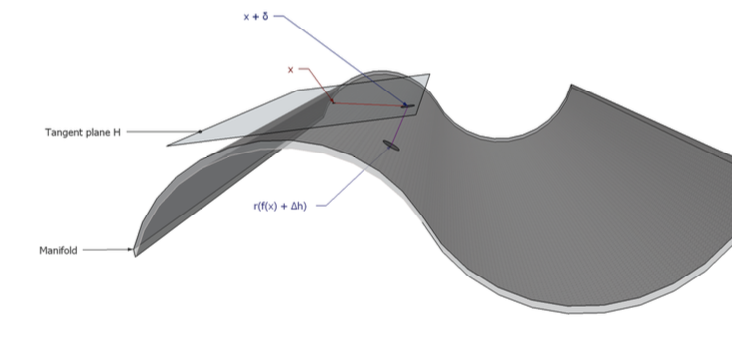
\includegraphics{images/2024-09-07-06-41-40.png}

}

\caption{a manifold in 3D space}

\end{figure}%

They list a bunch of priors about the data that have turned out to be
useful: smoothness, multiple explanatory factors, hierarchical
organization of factors, shared factors, manifolds, clustering,
sparsity.

\textbf{explaining away:} ``a priori independent causes of an event can
become non-independent given the observation of the event.'' Example:
you get notified that your burglar alarm went off, then you hear that
there was an earthquake. Your posteriors over being burgled and
earthquake now become tightly correlated.
\item[Kevin Murphy (2024)
\href{https://probml.github.io/pml-book/book1.html}{Probabilistic
Machine Learning}]
Good recent textbook with treatment of manifold hypothesis \& various
dimensionality-reduction \& manifold-learning algorithms.
\item[Generalized Low-Rank Models]
Udell et al.~(2016) ``Generalized Low Rank Models'': extension of PCA to
(1) any type of tabular data, not just scalars; (2) penalization of the
latent factors.

\begin{itemize}
\tightlist
\item
  Can be used to impute missing values.
\end{itemize}

\begin{itemize}
\item
  \begin{quote}
  ``low rank approximation problems are not convex, and in general
  cannot be solved globally and efficiently.''
  \end{quote}
\end{itemize}

\begin{itemize}
\tightlist
\item
  PCA: equivalently (1) find another matrix that is similar but has
  lower rank; (2) find a common basis of rows and columns, so that
  entries are products of embeddings.
\end{itemize}

\begin{itemize}
\tightlist
\item
  SVD: an exact decomposition into factors, then PCA is just truncation
  of the SVD factors. This is a way of analytically achieving a PCA
  solution, but for more complex cases need computable algorithms.
\end{itemize}

\begin{itemize}
\tightlist
\item
  Can interpret PCA as denoising: ``quadratically regularized PCA
  corresponds to a model in which features are observed with N(0,1)
  errors.''
\end{itemize}
\item[Markov blanket]
Given a set of random variables, a
\href{https://en.wikipedia.org/wiki/Markov_blanket}{Markov blanket} with
respect to a single variable \(Y\) is a subset that is collectively
sufficient to infer \(Y\).
\item[Inversion of embeddings]
@morris2023textembeddingsrevealalmost show that you can recover a string
from its embedding. They can perfectly recover 92\% of 32-token strings
from Wikipedia after they have been embedded into 1536 dimensions (using
OpenAI's production embedding).

Another paper by the same authors show that different embeddings all
match each other, so you can map them to each other without any labels.
\item[Information-Theoretic Framework]
Jeon, Zhu \& van Roy (2022) \href{https://arxiv.org/pdf/2203.00246}{``An
Information-Theoretic Framework for Supervised Learning''} -- seems
relevant. ``This prior distribution gives rise to high-dimensional
latent representations that, with high probability, admit reasonably
accurate low-dimensional approximations.''

Wilson (2025) \href{https://arxiv.org/pdf/2503.02113}{``Deep Learning is
Not So Mysterious or Different''} -- he argues that the ability for deep
networks to generalize is consistent with prior literature, specifically
that models have \emph{soft inductive biases} meaning a bias towards
simplicity.
\end{description}

\subsection{Related Economics
Literature}\label{related-economics-literature}

\begin{description}
\tightlist
\item[Rational inattention.]
(sims/caplin/woodford) is just about compressing a high-dimensional
signal to fit it through a pipeline, not about ignorance of the
distribution, or making inferences from it.
\item[Learning in games.]
Various people have written about Bayesian agents slowly learning the
state of the world, e.g.~Fudenberg and Levine on learning in games,
though I think those models are typically low-dimensional.
\item[Misspecified models.]
(Alwyn Young, Matt Rabin) -- but this is assuming it's low-dimensional
model. Maybe people have well-specified but imperfectly calibrated
models.
\item[Agreeing to disagree.]
Aumann. Presumably the speed of convergence is proportional to
complexity of the world models. If so then high-dimensional models could
rationalize the substantial equilibrium variance in beliefs. Might be
able to formalize this in Gaussian model.
\end{description}

\marginnote{\begin{footnotesize}

\begin{figure}[H]

{\centering \includegraphics{images/2023-11-02-10-44-49.png}

}

\caption{from Callender}

\end{figure}%

\end{footnotesize}}

\begin{description}
\tightlist
\item[Rugged landscape.]
Steven Callender has some papers, e.g.~``Innovation and Competition on a
Rugged Technological Landscape'', e.g.~see the graph in the margin.
\end{description}

\section{Misc}\label{misc-1}

\subsection{Short Version}\label{short-version}

Here's a big-picture take on econ modeling.

In short: we usually model agents making inferences given a
low-dimensional signal (n\textgreater p), but in fact maybe the more
common decision problem is high dimensional (n \textless{} p),
i.e.~people have plenty of signal but they don't know how to interpret
it.

Motivated by this observation: computers have been able to beat humans
at statistical inference since the 1960s for low-dimensional problems,
e.g.~linear regression (n\textgreater p), but it took another 50 years
for computers to learn how to do high-dimensional problems (n
\textless{} p), e.g.~to interpret text, images, and sound. An
implication is that humans must have some powerful modules for
interpreting high-dimensional data (AKA finding latent structures), \&
perhaps modeling that process is important for understanding
communication.

An additional observation: when we model decision-making under
uncertainty we usually assume the problem is low-dimensional
(n\textgreater p). We assume people already know the joint distribution
of everything (rational expectations), and their signal is coarse
relative to the state of the world, i.e.~they are constrained on p.~

But in reality signals don't seem so coarse: people read the newspaper,
they observe rich details about each others' behaviour, they have the
ability to examine products carefully. Maybe instead the problem is that
they have rich signals but they don't know how to interpret them,
i.e.~maybe the more common economic inference problem is
high-dimensional (p\textless n).

Some implications:

\begin{itemize}
\item
  In this world you can't reduce economic decision-making to a few
  variables: consumers make judgments using a \emph{gestalt} from rich
  data, so predicting behavior just using price and quality will have
  limited explanatory power (similarly, businesses don't just use
  interest rate \& unemployment to form expectations).
\item
  The value of more experience (doubling \(n\)) is higher than the value
  of a richer signal (doubling \(p\)).
\item
  Unsupervised learning is valuable, it helps you learn the latent
  structure of the world, thus agents with experience in one problem
  will be better at unrelated problems, e.g.~judging quality or
  forecasting economic conditions, because they have a stronger grasp of
  the latent structure of the world.
\end{itemize}

I know of a couple of things that are superficially similar but I think
don't quite capture this: rational inattention (sims/caplin/woodford) is
just about compressing a high-dimensional signal, not about ignorance of
the distribution; various people have written about Bayesian agents
slowly learning the state of the world (e.g.~Fudenberg and Levine on
learning in games) but I think those models are low-dimensional.

\subsection{Comments}\label{comments}

\textbf{Rob Donelly comments:}

\begin{quote}
``I agree with your claim that most of economic modeling has generally
focused on restricting the agents uncertainty to a low dimensional set
of signals, but I wonder how much of that is limitation of what is
tractable in a theory model (and similar constraints for an empirical
model).
\end{quote}

\begin{quote}
``For example Frank Knight had his paper about unknown/unquantifiable
risks back in 1921, but I don't think there has been much progress on
good approaches for modeling this. It's reasonably challenging to have a
model of uncertainty even with a single dimensional uncertainty
(e.g.~2001 Nobel prize for Akerlof, Spence, Stiglitz).
\end{quote}

\begin{quote}
``In empirical models it's especially difficult to try to learn what
someone's beliefs/expectations are, since we almost never have ground
truth data on beliefs, so instead we have to try to infer those beliefs
based on decisions. Usually that is only possible under very strong
modeling assumptions about what people know and what they are uncertain
about. At least in the consumer search models that I am most familiar
with, that usually ends up with a model where consumers have accurate
expectations/beliefs about nearly everything except for a very small
number of things they are learning/updating about.
\end{quote}

\begin{quote}
``It seems like the other extreme is a purely behavioral model e.g.~that
takes the entire lifetime history of everything a person has seen and
done, and predicts what'll they'll do/choose next.
\end{quote}

\begin{quote}
``A slightly different context, Athey has the paper that tries to
predict for timber auctions what will happen when they move from a open
bid to sealed bid auction. There she showed you can predict how the
buyers will respond to the new auction format by assuming their prior
behavior was generated under rational expectations + a single
dimensional type
\end{quote}

\begin{quote}
``It's unclear to me under what circumstances you would trust a purely
behaviorally grounded model to be able to extrapolate to new
circumstances that are very different than the data you trained on
\end{quote}

\textbf{Sean Taylor:}

\begin{quote}
``One concept I like for this is a''world model'' which the intelligent
agent uses to make predictions and choose actions. We are choosing
models and parameters which are analytically convenient or which make it
possible to identify the world model from data, but it's a much more
general concept \ldots{} I believe it is reinforcement learning
terminology.
\end{quote}

\subsection{Other Notes}\label{other-notes}

\textbf{Chemistry predicting properties of substances from atomic
structure.} It's better to predict behaviour from behaviour of other
macrophenomon, than to predict from microstructure.

\textbf{Application: forecasting.} Given the same information (the same
p) people have different experience (different n), and so substantially
different ability to forecast. In addition, in many cases people are
more constrained on having more history (base rates) than on knowing
more about this particular situation.

Also note that good forecasters can way outperform low-dimensional
statistical models, because the good forecasters have latent model of
the world.

\textbf{The mind and the computer are just reflections of the world.} We
can study the world, the mind, and the computer. But we will find the
same patterns reflected in all three.

\textbf{High-dimensional problems are the ones that used to be uniquely
the domain of humans.}

\emph{Application to perception:}

\begin{itemize}
\tightlist
\item
  Woodford will talk about how there's too much information, but then
  sets it up as a problem of \emph{compressing} the information to fit
  through a pipeline, rather than a problem of interpreting the
  information.
\end{itemize}

\begin{enumerate}
\def\labelenumi{\arabic{enumi}.}
\item
  \textbf{Humans have an uncanny ability to interpret high-dimensional
  data (n\textless\textless p).} Computers have been able to beat humans
  at low-dimensional prediction problems for 50 years. But only in the
  last 10 years have computers figured out how to interpret images,
  text, sound.
\item
  \textbf{Typical econ approach: you know distribution, form expectation
  E{[}v\textbar x{]}.} But
\end{enumerate}

\emph{A model of high-dimensional inference.}

\begin{itemize}
\tightlist
\item
  You get signal x=Av, where A is unknown.
\item
  You have x\_1,\ldots,x\_\{p-1\} and want to predict x\_p.
\item
  You have n prior experiences of x.
\end{itemize}

\emph{Applied to consumer choice:} purchase decision is \emph{gestalt},
not just price and unidimensional quality.

\textbf{Data generating process for high dimensional}

We want a generate model such that:

\begin{enumerate}
\def\labelenumi{\arabic{enumi}.}
\tightlist
\item
  Low dimensional state generates high-dimensional signal.
\item
  The state \emph{cannot} be recovered with a simple algorithm (linear,
  nearest neighbor). You need something hierarchical like a neural net.
\end{enumerate}

Examples:

\begin{itemize}
\tightlist
\item
  \emph{2D view of 3D scene.} this has both (i) big interactions,
  e.g.~green object looks cyan when the light is blue; (ii) complex
  environmental statistics -- you need to gradually learn priors.
\end{itemize}

\textbf{Perception wrongly treated as compression.} It's clear in many
cases of perception that the signal is high-dimensional, yet there are
some weird anomalies. A common model is that the signal is
\emph{compressed} and then reconstructed. E.g. Sim, Woodford, compressed
sensing, etc. The \emph{compression} problem has some subtle differences
from the \emph{inference} problem.

\begin{description}
\tightlist
\item[Could call the states ``noumena'' and the signals ``phenomena''.]
asfd
\end{description}

\section{2025-02-17 \textbar{} causal view vs manifold
view}\label{causal-view-vs-manifold-view}

\begin{description}
\item[Causal inference people are skeptical about LLMs.]
Susan Athey seems to think that LLMs are fundamentally limited because
they're just next-word predictors, there's no allowance for causal
inference.{[}3{]}

\href{https://www.youtube.com/live/W0QLq4qEmKg?t=3810s}{Michael Jordan}
says \emph{``I don't think there's ever been an era in human history
where a new field of technology has arisen where there was so much hype
and hysteria around it''}
\item[LLM people \emph{sound} like they're making classic mistakes.]
The things that LLM people say are things that make causal-inference
people roll their eyes. They say \emph{``we just need more data''}, and
\emph{``we just need a better functional form''} which are exactly the
things that people say when they are doing supervised learning which
will yield confounded causal estimates. It's also true that most LLM
people have only a vague understanding of causal inference techniques.
\item[Despite this, LLMs are working anyway.]
Despite all this LLMs are clearly very useful, they can do a huge
variety of tasks autonomously, and there's a huge demand for people to
use them to help solve problems. Their abilities are expanding rapidly.
\item[I think there's a deep disagreement about knowledge.]
Here are two simplified ways of characterizing knowledge about the
world:

\begin{enumerate}
\def\labelenumi{\arabic{enumi}.}
\item
  \emph{We are learning parameters.} E.g. we are slowly learning the
  causal effects of different medicines, learning the elasticities of
  demand, learning the returns to education. This is the causal
  inference worldview. There set of parameters are small. Progress comes
  from doing experiments and gradually mapping out the world better.
\item
  \emph{We are learning structures.} We are learning how to
  \emph{factorize} a high dimensional world into low dimensions. E.g.
  (1) we learn to exlpain the motions of the stars with a heliocentric
  model, (2) we explain physical interactions with mass and momentum;
  (3) we categorize medical conditions with temperature, blood pressure,
  pulse; (4) we categorize economic conditions with GDP, inflation,
  employment.
\end{enumerate}
\item[The causal inference worldview is narrow.]
The textbook causal inference worldview is focussed on learning causal
parameters. The classical case is when you have a low-dimensional
dataset (\(n>p\)) and you are identifying some causal parameter of
interest using an experiment or natural experiment. Then we can think of
decision-makers as gradually updating their beliefs about causal effects
using causal inference, e.g.~updating price elasticities, or updating
estimates of the returns to education. However this worldview has some
problems:

\begin{enumerate}
\def\labelenumi{\arabic{enumi}.}
\item
  \emph{In most circumstances there is no identifying variation.}
  Despite this people clearly have good causal knowledge, enough to cure
  diseases and build nation-states and aeroplanes and skyscrapers.
  Another way of making this point: our economic models usually assume
  that decision-makers know the true causal effects, yet econometricians
  say that they can't figure the causal effects out themselves.
\item
  \emph{Almost all real-world datasets are high dimensional} (\(p>n\)),
  so there's necessarily some dimensionality-reduction before we can
  estimate a causal effect.
\item
  \emph{There's little reason to expect causal coefficients to be
  stable.} Economists talk about coefficients as ``the'' return to this
  or that, but often glide over how realistic it is that these be
  stable.
\item
  Most history of progress in science is more about discovering new
  regularities, than about better estimates of causal coefficients.
\end{enumerate}
\item[There's an alternative vision.]
(\ldots)
\end{description}

\subsection{Background}\label{background}

I think their skepticism is because LLMs look like a mistake they've
seen before.

\subsection{The Causal Worldview and its
Problems}\label{the-causal-worldview-and-its-problems}

\begin{description}
\tightlist
\item[This is a caricture of the worldview implicit in the ``causal
inference'' approach.]
\item[We have a low-dimensional dataset (n\textgreater p)]
E.g. a set of country-year pairs and macroeconomic variables, or
state-year pairs and social variables, or person-year pairs and health
variables.
\item[Bad science is correlations, good science is causation.]
Bad science is finding correlations between variables and interpreting
them causally. E.g. bad public health,
\item[The goal is to find the few true causal effects.]
E.g. we want to estimate the fiscal multiplier, or the coefficient of
relative risk aversion, or the returns to education.
\end{description}

\subsection{Problems with the Causal
Worldview}\label{problems-with-the-causal-worldview}

2023:
\href{https://www.promarket.org/2023/07/08/a-conversation-with-susan-athey/}{``A
Conversation with Susan Athey''}

\begin{enumerate}
\def\labelenumi{\arabic{enumi}.}
\tightlist
\item
  \emph{View of the world:} there are a small number of causal effects
  we need to estimate (elasticities).
\item
  \emph{The hard part is the dimension-reduction.}
\item
  \emph{Dimension reduction in physics} - temperature, center of mass,
  momentum, mass, pressure, charge, spin, angular momentum, rate of
  flow.
\end{enumerate}

\subsection{Some concrete
applications}\label{some-concrete-applications}

\begin{enumerate}
\def\labelenumi{\arabic{enumi}.}
\tightlist
\item
  We want to grow our crops better.
\item
  We want to .
\end{enumerate}

\subsection{Summary for Zoe \& Chris}\label{summary-for-zoe-chris}

Chris and I were talking about Susan Athey's skepticism of AI (Mike
Jordan has a very similar attitude). Here's my very big picture take.

First: I think Susan Athey's bullshit detector goes off when she hears
about LLMs, because she's so used to seeing people confuse supervised
learning and causal inference. So she feels comfortable dismissing a lot
of the claims about LLMs because she thinks she knows why they're
confused.

In fact there are two polar views of scientific progress:

\begin{enumerate}
\def\labelenumi{\arabic{enumi}.}
\tightlist
\item
  \emph{Learning parameters.} We're slowly mapping out the world with
  experiments. We're bottlenecked on having more causal data.
\item
  \emph{Learning structures.} We're slowly \emph{understanding} the
  world by finding latent structure, i.e.~reducing high-dimensional
  world to low-dimensional. We're not primarily bottlenecked on having
  more causal data. However it can be useful to have unsupervised data
  to learn the mapping from high-dimensional to low-dimensional
  (technically LLM pretraining is supervised but in a narrow sense).
\end{enumerate}

Economists have become very fixated on the ``learning parameters''
worldview, especially post-credibility-revolution.

However in fact almost all scientific and technological progress is
\emph{not} from learning parameters, but instead from learning
structures. Most progress comes from factorizing the world into a
low-dimensional structure. The reason NNs \& LLMs are revolutionary is
that we've finally taught computers to do that low-dimensional
factorization themselves, \& now they can reason about the world.

\section{2025-03-06 \textbar{} Everything is downstream of the
statistical structure of the
world.}\label{everything-is-downstream-of-the-statistical-structure-of-the-world.}

\begin{description}
\tightlist
\item[Everything is downstream of the statistical structure of the
world.]
Economists say that everything is determined by the production function.
But the production function for knowledge work is determined by the
statistical structure of the world, so that's what everything's truly
downstream of.

\begin{itemize}
\tightlist
\item
  If the world is highly repetitive, the returns to experience are
  small, and the returns to firm scale are small.
\end{itemize}

\begin{itemize}
\tightlist
\item
  If the world is highly idiosyncratic, then returns to experience are
  small.
\end{itemize}

\begin{itemize}
\tightlist
\item
  But if the world has deep latent structure, then the returns to
  experience are high.
\end{itemize}

Applications:

\begin{itemize}
\tightlist
\item
  \emph{High returns to experience in medicine.}
\end{itemize}

\begin{itemize}
\tightlist
\item
  \emph{Google gets high margins because returns to information remain
  high at that scale}
\end{itemize}

\begin{itemize}
\tightlist
\item
  \emph{Margins in AI will depend on structure of the world.}
\end{itemize}
\end{description}

\section{2025-07-17 \textbar{}}\label{section}

Huh et al.~(2025) \href{https://arxiv.org/abs/2405.07987}{The Platonic
Representation Hypothessis}

Jack Morris (2025)
\href{https://blog.jxmo.io/p/there-is-only-one-model}{All Models Might
be the Same}




\end{document}
